\chapter{Linear Models for Classification}
\label{ch:classification}

\chapterguide%
  {\chapref{ch:supervised}, \chapref{ch:training}, and probability/odds from \chapref{ch:statistics}.}
  {Fit and interpret logistic regression, extend it to many classes with softmax, explain how discriminant analysis reaches a linear boundary from a different direction, recognize ordered-category labels, and place the perceptron in its historical role.}

Classification asks the model to choose a category. The simplest useful family of classifiers draws a straight line (in higher dimensions, a flat plane) through feature space and predicts one class on each side. This chapter covers the three classical ways to find that line: logistic regression, discriminant analysis, and the perceptron.

\begin{firstread}
Core path: logistic regression, cross-entropy, decision thresholds, and softmax regression. Ordinal labels are a useful special case. LDA and the perceptron are comparison models for a second pass rather than prerequisites for later chapters.
\end{firstread}

\section{Why not just use linear regression?}

A tempting shortcut is to represent the classes as $y\in\{0,1\}$ and fit ordinary least squares. It fails in two instructive ways: the model happily predicts values like $-0.3$ or $1.7$, which cannot be probabilities, and squared error punishes the model for being \emph{too correct} --- an extremely obvious positive example far from the boundary pulls the line toward itself just as an outlier would. Classification needs an output that lives in $[0,1]$ and a loss that rewards confident correct answers.

\section{From probabilities to odds to a linear model}

If an event has probability $p$, its \term{odds} are $p/(1-p)$: a probability of $0.75$ means odds of $3$ (``three to one''). Odds run from $0$ to infinity, and their logarithm --- the \term{log-odds} or \term{logit} --- runs over the whole real line. Logistic regression makes one clean assumption: \emph{the log-odds are a linear function of the features},

\begin{mltable}
\begin{tabularx}{0.78\linewidth}{@{}>{\bfseries\leavevmode\color{MLNavy}}X X X@{}}
\toprule
\rowcolor{MLPaleBlue!92}
Probability & Odds & Read aloud \\
\midrule
$50\%$ & $1:1$ & equally likely either way \\
$75\%$ & $3:1$ & three chances for, one against \\
$90\%$ & $9:1$ & nine chances for, one against \\
\bottomrule
\end{tabularx}
\end{mltable}

Logistic regression uses log-odds because an unrestricted score can then be converted into a valid probability between 0 and 1. You do not normally calculate the logarithm by hand; the library performs the conversion.

\[
  \log\frac{p}{1-p}
  =\beta_0+\bm{\beta}^{\mathsf T}\bm{x}.
\]
Solving for $p$ inverts the logarithm and produces the familiar S-shaped \term{sigmoid}:
\[
  P(Y=1\given\bm{x})
  =\sigma(z)
  =\frac{1}{1+e^{-z}},
  \qquad
  z=\beta_0+\bm{\beta}^{\mathsf T}\bm{x}.
\]

\begin{mlfigure}
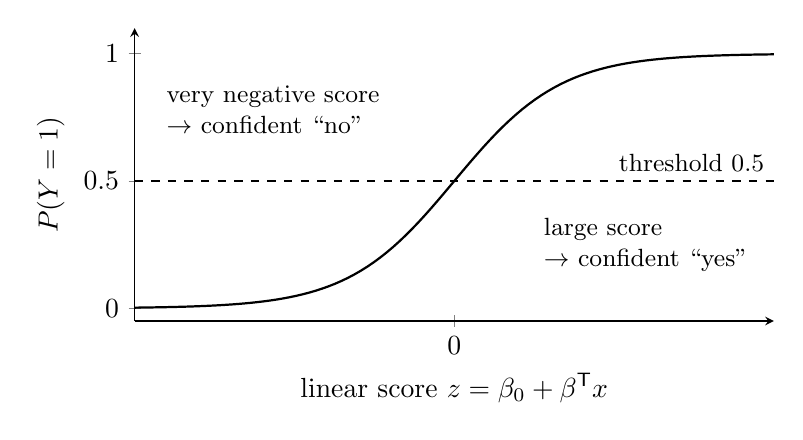
\begin{tikzpicture}
\begin{axis}[
  width=0.80\linewidth, height=5.3cm,
  axis lines=left,
  xlabel={linear score $z=\beta_0+\bm{\beta}^{\mathsf T}\bm{x}$},
  ylabel={$P(Y=1)$},
  ytick={0,0.5,1}, xtick={0},
  domain=-6:6, samples=100, ymin=-0.05, ymax=1.1, clip=false
]
\addplot[thick] {1/(1+exp(-x))};
\draw[dashed] (axis cs:-6,0.5) -- (axis cs:6,0.5)
  node[above left, font=\small] {threshold $0.5$};
\node[font=\small, align=left] at (axis cs:3.6,0.25) {large score\\$\rightarrow$ confident ``yes''};
\node[font=\small, align=left] at (axis cs:-3.4,0.78) {very negative score\\$\rightarrow$ confident ``no''};
\end{axis}
\end{tikzpicture}
\end{mlfigure}

\begin{intuition}
The sigmoid is a ``squashing'' function: it takes any score, from minus infinity to plus infinity, and gently bends it into the range $0$ to $1$ so it can be read as a probability. Scores near zero mean the model is unsure; scores far from zero mean it is confident.
\end{intuition}

The coefficients have a crisp interpretation: increasing $x_j$ by one unit multiplies the odds by $e^{\beta_j}$. A coefficient of $0.7$ roughly doubles the odds ($e^{0.7}\approx 2.01$); a coefficient of $-0.7$ roughly halves them.

\begin{workedexample}
Suppose a pass/fail model based on hours studied has $\beta_0=-4$ and $\beta_1=0.08$.
A student with $x=60$ hours has score $z=-4+0.08\times 60=0.8$ and pass probability $\sigma(0.8)\approx 0.69$.
A student with $x=30$ hours has $z=-1.6$ and $\sigma(-1.6)\approx 0.17$.
Each additional hour multiplies the odds of passing by $e^{0.08}\approx 1.083$ --- about an $8\%$ increase in the odds, regardless of the starting point.
\end{workedexample}

\section{Training with cross-entropy}

For binary classification with predicted probability $p$, the loss for one observation is the \term{cross-entropy} (equivalently, the negative log-likelihood of a Bernoulli model from \chapref{ch:statistics}):
\[
  \mathcal{L}(y,p)
  =-[y\log p+(1-y)\log(1-p)].
\]
When $y=1$ the loss is $-\log p$: near zero if the model was confident and right, and enormous if the model was confident and wrong. The gradient of the average loss has a strikingly simple form,
\[
  \nabla_{\bm{\beta}}J
  =\frac{1}{n}\sum_{i=1}^{n}(p_i-y_i)\,\bm{x}_i,
\]
so each update is driven directly by the prediction error $p_i-y_i$. There is no closed-form solution; the parameters are found by iterative optimization such as gradient descent or Newton-type methods (\chapref{ch:training}). With the usual convex objective and an appropriate solver, optimization is not trapped by inferior local minima.

\subsection{The decision boundary and the threshold}

Predicting class $1$ whenever $p\geq 0.5$ is the same as predicting class $1$ whenever the score $z\geq 0$, so the boundary between the classes is the flat surface $\beta_0+\bm{\beta}^{\mathsf T}\bm{x}=0$ --- hence ``linear'' classifier. The threshold need not stay at $0.5$: when a missed positive costs more than a false alarm, a lower threshold may be appropriate; in the opposite case a higher one may be. \chapref{ch:evaluation} shows how to choose it with validation or out-of-fold predictions.

\subsection{Regularization}

Exactly as in \chapref{ch:regression}, an $L_2$ or $L_1$ penalty on $\bm{\beta}$ controls overfitting when features are numerous or correlated. Features should usually be standardized before coefficient penalties are compared, the penalty strength is tuned on validation data, and regularization also cures a quirk of the unpenalized model: on perfectly separable data, plain logistic regression pushes its coefficients toward infinity chasing ever-more-confident probabilities.

\section{Softmax regression for multiple classes}

For $K$ classes, each class $k$ receives its own weight vector, and the \term{softmax} function converts the $K$ linear scores into probabilities:
\[
  P(Y=k\given\bm{x})
  =\frac{\exp(\bm{\beta}_k^{\mathsf T}\bm{x})}
        {\sum_{j=1}^{K}\exp(\bm{\beta}_j^{\mathsf T}\bm{x})}.
\]
Each class's score is exponentiated (making it positive) and divided by the total (making the probabilities sum to one); the largest score wins the largest probability. Training minimizes the multiclass cross-entropy $\mathcal{L}=-\log P(Y=y\given\bm{x})$, the direct generalization of the binary loss.

A simpler alternative that works with any binary classifier is \term{one-vs-rest}: train $K$ separate binary models (``class $k$ against everything else'') and predict the class whose model is most confident.

\section{Ordered categories are not ordinary multiclass labels}
\label{sec:ordinal-labels}

Some labels are categories with a meaningful order: \emph{low $<$ medium $<$ high}, satisfaction ratings, or disease stages. This is an \term{ordinal} label. Ordinary softmax classification ignores the order, while coding the labels as $1,2,3$ and using ordinary regression invents equal numerical gaps that may not exist.

\begin{mltable}
\begin{tabularx}{\linewidth}{@{}p{0.25\linewidth}X@{}}
\toprule
\rowcolor{MLPaleBlue!92}
Approach & When it makes sense \\
\midrule
Ordinary multiclass classifier & Use when categories are genuinely unordered or when order is irrelevant to the decision. \\
Ordinal model / order-aware loss & Prefer when confusing adjacent levels is meaningfully less serious than confusing the two extremes. \\
Regression on integer codes & Use only when the numerical spacing itself is defensible; do not use it merely because the labels can be numbered. \\
\bottomrule
\end{tabularx}
\end{mltable}

There is no single universally appropriate model for ordinal labels. The important first-course skill is recognizing the ordered label structure and choosing an order-aware method or metric when the application requires it. Validation still decides whether that added structure improves the real task.

\section{Linear discriminant analysis}

Logistic regression is a \term{discriminative} model: it learns $P(y\given\bm{x})$ directly and never asks what the features of each class look like. \term{Linear discriminant analysis (LDA)} takes the opposite, \term{generative} route: model what each class's data looks like, then use Bayes' theorem to classify.

LDA assumes each class $k$ generates its features from a Gaussian with its own mean $\bm{\mu}_k$ but a \emph{shared} covariance matrix $\Sigma$, and that class $k$ occurs with prior probability $\pi_k$. Bayes' theorem then assigns a new point to the class with the largest \term{discriminant score}
\[
  \delta_k(\bm{x})
  =\bm{x}^{\mathsf T}\Sigma^{-1}\bm{\mu}_k
  -\tfrac{1}{2}\bm{\mu}_k^{\mathsf T}\Sigma^{-1}\bm{\mu}_k
  +\log\pi_k.
\]
Every term is estimated by counting and averaging: $\pi_k$ from class frequencies, $\bm{\mu}_k$ from class means, and $\Sigma$ from pooled within-class spread. Because $\bm{x}$ enters only linearly, the boundary between any two classes is again a straight line --- LDA and logistic regression draw the same \emph{kind} of boundary, found by different reasoning.

\begin{intuition}
Picture two hills of sand of identical shape, one centered on each class's average, scaled by how common each class is. LDA classifies a new point by asking which hill stands taller at that spot. With identically shaped hills, the tie line between them is straight --- and it shifts toward the rarer class, since its hill is lower everywhere.
\end{intuition}

When to prefer which:

\begin{itemize}
  \item LDA estimates its parameters in one pass with simple formulas, so it is fast and remarkably stable on \emph{small} datasets --- when its Gaussian assumption is roughly right, it can beat logistic regression there.
  \item Logistic regression assumes less about the features and is more robust when classes are far from Gaussian (heavy tails, strong outliers, many binary features).
  \item LDA doubles as a supervised dimensionality-reduction method: for $K$ classes it finds up to $K-1$ directions that best separate them, a useful companion to PCA (\chapref{ch:dimred}).
\end{itemize}

\term{Quadratic discriminant analysis (QDA)} drops the shared-covariance assumption and gives each class its own $\Sigma_k$. The boundaries become curved (quadratic), which is more flexible but requires estimating many more parameters --- QDA needs considerably more data per class to stay reliable.

\section{The perceptron}

The \term{perceptron} (1958) is the historical ancestor of this whole family. It predicts with the sign of a linear score, $\hat{y}=\operatorname{sign}(\bm{w}^{\mathsf T}\bm{x}+b)$ with $y\in\{-1,+1\}$, and learns by an appealingly simple rule: visit the training examples one at a time, and whenever one is misclassified, nudge the boundary toward it,
\[
  \bm{w}\leftarrow\bm{w}+\eta\,y_i\,\bm{x}_i,
  \qquad
  b\leftarrow b+\eta\,y_i.
\]
Correctly classified points cause no update at all. If the classes are linearly separable, the perceptron is guaranteed to find a separating boundary in finitely many mistakes; if they are not, the basic algorithm need not settle down. It outputs no probabilities, and among the many separating lines it stops at one determined by the update path. Logistic regression and the support vector machine (\chapref{ch:svm}) address these weaknesses differently --- one models probabilities, while the other maximizes a margin.

\section{Choosing among linear classifiers}

\begin{mltable}
\begin{tabular}{@{}p{0.22\linewidth}p{0.34\linewidth}p{0.34\linewidth}@{}}
\toprule
\rowcolor{MLPaleBlue!92}
Model & Useful strengths & Important limitations \\
\midrule
Logistic regression & Strong probability baseline, convex training, interpretable odds ratios & Linear boundary; probabilities can still be miscalibrated under misspecification or shift \\
LDA & Very fast, stable on small data, gives class-separating directions & Assumes Gaussian classes with shared covariance \\
QDA & Curved boundaries, per-class covariance & Many parameters; needs much more data \\
Perceptron & Simplest possible trainer; historically important & No probabilities; unreliable when classes overlap \\
\bottomrule
\end{tabular}
\end{mltable}

\begin{keyidea}
Logistic regression, LDA, and the perceptron separate classes with flat boundaries, but choose those boundaries differently. Logistic regression maximizes the conditional likelihood; LDA models each class and applies Bayes' theorem; the perceptron nudges a line after each mistake and may not settle when classes overlap. QDA is the exception here: separate class covariances produce curved boundaries. The coming chapters add other forms of nonlinearity through neighborhoods, trees, ensembles, and kernels.
\end{keyidea}

\begin{modelcard}{Linear Classifiers - Quick Guide}
\begin{tabularx}{\linewidth}{@{}>{\bfseries\leavevmode\color{MLNavy}}p{0.24\linewidth}X@{}}
Best when & A linear boundary is reasonable, fast prediction matters, or coefficients need to be interpreted. \cr
Start with & Logistic regression for probabilities; softmax regression for several classes. \cr
Preprocessing & Encode categories, standardize numerical features for regularization, and handle imbalance with suitable metrics or weights. \cr
Main controls & Regularization strength, penalty type, and the probability threshold used for decisions. \cr
Watch for & Nonlinear class structure, poorly calibrated probabilities, rare classes, and causal over-interpretation (\secref{sec:correlation}). \cr
\end{tabularx}
\end{modelcard}

\section{Using linear classifiers in practice}
\label{sec:logistic-practice}

\subsection{Probabilities, not just labels}

\subsection{Moving the threshold on purpose}

\begin{intuition}
Read the table as a dial, not a set of separate models. It is a single trained model being asked to be more or less cautious. A cancer screening service would choose the top row and accept the false alarms. A system that automatically freezes bank accounts would choose the bottom row, because wrongly freezing an account is expensive.
\end{intuition}

Choose the operating point from out-of-fold predictions and a stated cost or capacity constraint. Then refit the model on all training data and assess that locked rule on the test set once.

\subsection{Reading the coefficients}

\begin{workedexample}
Suppose the coefficient for ``hours studied'' is $0.62$. Then $e^{0.62}\approx 1.86$. Interpretation: each extra hour of study multiplies the \emph{odds} of passing by about 1.86 --- roughly an 86\% increase in the odds, holding the other features fixed. Note that this is odds, not probability; the effect on probability depends on where you started.
\end{workedexample}

\subsection{More than two classes}

\begin{mlfigure}
\begin{tikzpicture}[
  node distance=0.36cm and 0.62cm,
  sc/.style={draw=MLBlue,fill=MLPaleBlue,rounded corners=1.2mm,minimum width=1.55cm,minimum height=0.6cm,align=center,font=\scriptsize\color{MLNavy}},
  pr/.style={draw=MLGreen,fill=MLPaleTeal,rounded corners=1.2mm,minimum width=1.55cm,minimum height=0.6cm,align=center,font=\scriptsize\color{MLNavy}},
  arr/.style={-{Stealth[length=2mm]},thick,draw=MLTeal}
]
\node[sc] (s1) {cat: $1.2$};
\node[sc,below=of s1] (s2) {dog: $3.4$};
\node[sc,below=of s2] (s3) {fox: $2.0$};
\node[draw=MLOrange,fill=MLPaleOrange,rounded corners=2mm,minimum height=2.5cm,minimum width=1.9cm,align=center,font=\scriptsize\bfseries\color{MLNavy},right=1.0cm of s2] (sm) {softmax\\[0.15em]\scriptsize\mdseries exponentiate,\\then divide by\\the total};
\node[pr,right=1.0cm of sm] (p2) {dog: $0.75$};
\node[pr,above=of p2] (p1) {cat: $0.08$};
\node[pr,below=of p2] (p3) {fox: $0.17$};
\draw[arr] (s1.east) -- (sm.west); \draw[arr] (s2.east) -- (sm.west); \draw[arr] (s3.east) -- (sm.west);
\draw[arr] (sm.east) -- (p1.west); \draw[arr] (sm.east) -- (p2.west); \draw[arr] (sm.east) -- (p3.west);
\node[font=\scriptsize\itshape\color{MLMuted},below=0.3cm of p3] {always adds to 1.00};
\end{tikzpicture}
\end{mlfigure}

\begin{keyidea}
Softmax is the sigmoid's multi-class cousin. It takes one raw score per class, makes them all positive by exponentiating, and then divides by the total so the results form a genuine probability distribution. The largest score always becomes the largest probability, but softmax also tells you \emph{how much} larger.
\end{keyidea}

\begin{tryit}
Fit a logistic regression, obtain out-of-fold probabilities on the training data, then sweep the threshold from 0.05 to 0.95 in steps of 0.05, recording precision and recall at each point. Plot recall on the $x$-axis against precision on the $y$-axis. You have just drawn a precision-recall curve by hand, as introduced in \chapref{ch:evaluation}, without using the test set.
\end{tryit}

\begin{debugtask}
A teammate lowers the probability threshold until test-set recall reaches the desired value, then reports that same test recall as final performance. Explain the leakage in model selection and show where threshold tuning belongs instead.
\end{debugtask}

\begin{decisionmemo}
For a rare positive class, choose between an unweighted logistic model, class weighting, and a lower decision threshold. State which quantity each intervention changes, which validation metric you would inspect, and why the three options are not interchangeable.
\end{decisionmemo}


\begin{quickcheck}
\begin{enumerate}
  \item Why is logistic regression called a linear classifier even though it outputs a nonlinear sigmoid probability?
  \item Why should the probability model and the operational classification threshold be treated as separate objects?
  \item What changes when binary logistic regression is extended to a multiclass softmax model?
\end{enumerate}
\end{quickcheck}

\begin{chapterrecap}
\begin{itemize}
  \item Logistic regression turns a linear score into a probability with the sigmoid function.
  \item The decision threshold converts a probability into a class and can be changed to match error costs.
  \item Cross-entropy strongly penalizes confident wrong predictions.
  \item Softmax regression extends the idea to multiple classes.
  \item LDA uses a probability model for each class; the perceptron learns a separating boundary but not probabilities.
\end{itemize}
\end{chapterrecap}
